\par $S = [6,6]$
\par $H(S) = -\frac{6}{12} \log_2 \frac{6}{12}-\frac{6}{12} \log_2 \frac{6}{12} = 1$

\vskip 0.3in
\par $S_{alternativa^+} = [3,3]$ \qquad $S_{alternativa^-} = [3,3]$
\par $H(S_{alternativa^+}) = -\frac{3}{6} \log_2 \frac{3}{6}- \frac{3}{6} \log_2 \frac{3}{6} = 1$
\par $H(S_{alternativa^-}) = -\frac{3}{6} \log_2 \frac{3}{6}- \frac{3}{6} \log_2 \frac{3}{6} = 1$
\par $Ganho(S, S_{alternativa}) = 1-\frac{6}{12} * 1-\frac{6}{12} * 1 = 0$

\vskip 0.3in
\par $S_{bar^+} = [3,3]$ \qquad $S_{bar^-} = [3,3]$
\par $H(S_{bar^+}) = -\frac{3}{6} \log_2 \frac{3}{6}- \frac{3}{6} \log_2 \frac{3}{6} = 1$
\par $H(S_{bar^-}) = -\frac{3}{6} \log_2 \frac{3}{6}- \frac{3}{6} \log_2 \frac{3}{6} = 1$
\par $Ganho(S, S_{bar}) = 1-\frac{6}{12} * 1-\frac{6}{12} * 1 = 0$

\vskip 0.4in
\par $S_{fimSemana^+} = [2,3]$ \qquad $S_{fimSemana^-} = [4,3]$
\par $H(S_{fimSemana^+}) = -\frac{2}{5} \log_2 \frac{2}{5}- \frac{3}{5} \log_2 \frac{3}{5} = 0.971$
\par $H(S_{fimSemana^-}) = -\frac{4}{7} \log_2 \frac{4}{7}- \frac{3}{7} \log_2 \frac{3}{7} = 0.985$
\par $Ganho(S, S_{fimSemana}) = 1.000-\frac{5}{12} * 0.971 -\frac{7}{12} * 0.985 = 0.021$

\vskip 0.3in
\par $S_{fome^+} = [5,2]$ \qquad $S_{fome^-} = [1,4]$
\par $H(S_{fome^+}) = -\frac{5}{7} \log_2 \frac{5}{7}- \frac{2}{7} \log_2 \frac{2}{7} = 0.863$
\par $H(S_{fome^-}) = -\frac{1}{5} \log_2 \frac{1}{5}- \frac{4}{5} \log_2 \frac{4}{5} = 0.722$
\par $Ganho(S, S_{fome}) = 1.000-\frac{7}{12} * 0.863-\frac{5}{12} * 0.722 = 0.196$

\vskip 0.3in
\par $S_{clientes^{alguns}} = [4,0]$ \qquad $S_{clientes^{cheio}} = [2,4]$\par $S_{clientes^{nenhum}} = [0,2]$
\par $H(S_{clientes^{alguns}}) = -\frac{4}{4} \log_2 \frac{4}{4}- \frac{0}{4} \log_2 \frac{0}{4} = 0.000$
\par $H(S_{clientes^{cheio}}) = -\frac{2}{6} \log_2 \frac{2}{6}- \frac{4}{6} \log_2 \frac{4}{6} = 0.918$
\par $H(S_{clientes^{nenhum}}) = -\frac{0}{2} \log_2 \frac{0}{2}- \frac{2}{2} \log_2 \frac{2}{2} = 0.000$
\par $Ganho(S, S_{clientes}) = 1.000-\frac{4}{12} * 0.000-\frac{6}{12} * 0.918-\frac{2}{12} * 0.000 = 0.541$

\vskip 0.3in
\par $S_{preço^{\$}} = [3,4]$ \qquad $S_{preço^{\$\$}} = [2,0]$\par $S_{preço^{\$\$\$}} = [1,2]$
\par $H(S_{preço^{\$}}) = -\frac{3}{7} \log_2 \frac{3}{7}- \frac{4}{7} \log_2 \frac{4}{7} = 0.985$
\par $H(S_{preço^{\$\$}}) = -\frac{2}{2} \log_2 \frac{2}{2}- \frac{0}{2} \log_2 \frac{0}{2} = 0.000$
\par $H(S_{preço^{\$\$\$}}) = -\frac{1}{3} \log_2 \frac{1}{3}- \frac{2}{3} \log_2 \frac{2}{3} = 0.918$
\par $Ganho(S, S_{preço}) = 1.000-\frac{7}{12} * 0.985-\frac{2}{12} * 0.000-\frac{3}{12} * 0.918 = 0.196$

\vskip 0.3in
\par $S_{chuva^{+}} = [3,2]$ \qquad $S_{chuva^{-}} = [3,4]$
\par $H(S_{chuva^{+}}) = -\frac{3}{5} \log_2 \frac{3}{5}- \frac{2}{5} \log_2 \frac{2}{5} = 0.971$
\par $H(S_{chuva^{-}}) = -\frac{3}{7} \log_2 \frac{3}{7}- \frac{4}{7} \log_2 \frac{4}{7} = 0.985$
\par $Ganho(S, S_{chuva}) = 1.000-\frac{5}{12} * 0.971-\frac{7}{12} * 0.985 = 0.021$

\vskip 0.3in
\par $S_{reserva^{+}} = [3,2]$ \qquad $S_{reserva^{-}} = [3,4]$
\par $H(S_{reserva^{+}}) = -\frac{3}{5} \log_2 \frac{3}{5}- \frac{2}{5} \log_2 \frac{2}{5} = 0.971$
\par $H(S_{reserva^{-}}) = -\frac{3}{7} \log_2 \frac{3}{7}- \frac{4}{7} \log_2 \frac{4}{7} = 0.985$
\par $Ganho(S, S_{reserva}) = 1.000-\frac{5}{12} * 0.971-\frac{7}{12} * 0.985 = 0.021$

\vskip 0.3in
\par $S_{reserva^{Francês}} = [1,1]$ \qquad $S_{reserva^{Tailandês}} = [2,2]$\par $S_{reserva^{Italiano}} = [1,1]$ \qquad $S_{reserva^{Hamburger}} = [2,2]$
\par $H(S_{reserva^{Francês}}) = -\frac{1}{2} \log_2 \frac{1}{2}- \frac{1}{2} \log_2 \frac{1}{2} = 1.000$
\par $H(S_{reserva^{Tailandês}}) = -\frac{2}{4} \log_2 \frac{2}{4}- \frac{2}{4} \log_2 \frac{2}{4} = 1.000$
\par $H(S_{reserva^{Italiano}}) = -\frac{1}{2} \log_2 \frac{1}{2}- \frac{1}{2} \log_2 \frac{1}{2} = 1.000$
\par $H(S_{reserva^{Hamburger}}) = -\frac{2}{4} \log_2 \frac{2}{4}- \frac{2}{4} \log_2 \frac{2}{4} = 1.000$
\par $Ganho(S, S_{reserva}) = 1.000-\frac{2}{12} * 1.000-\frac{4}{12} * 1.000-\frac{2}{12} * 1.000-\frac{4}{12} * 1.000 = 0.000$


\vskip 0.3in
\par $S_{reserva^{0-10}} = [4,2]$ \qquad $S_{reserva^{10-30}} = [1,1]$\par $S_{reserva^{30-60}} = [1,1]$ \qquad $S_{reserva^{>60}} = [0,2]$
\par $H(S_{reserva^{0-10}}) = -\frac{4}{6} \log_2 \frac{4}{6}- \frac{2}{6} \log_2 \frac{2}{6} = 0.918$
\par $H(S_{reserva^{10-30}}) = -\frac{1}{2} \log_2 \frac{1}{2}- \frac{1}{2} \log_2 \frac{1}{2} = 1.000$
\par $H(S_{reserva^{30-60}}) = -\frac{1}{2} \log_2 \frac{1}{2}- \frac{1}{2} \log_2 \frac{1}{2} = 1.000$
\par $H(S_{reserva^{>60}}) = -\frac{0}{2} \log_2 \frac{0}{2}- \frac{2}{2} \log_2 \frac{2}{2} = 0.000$
\par $Ganho(S, S_{reserva}) = 1.000-\frac{6}{12} * 0.918-\frac{2}{12} * 1.000-\frac{2}{12} * 1.000-\frac{2}{12} * 0.000 = 0.208$

\vskip 0.4in
\hfil
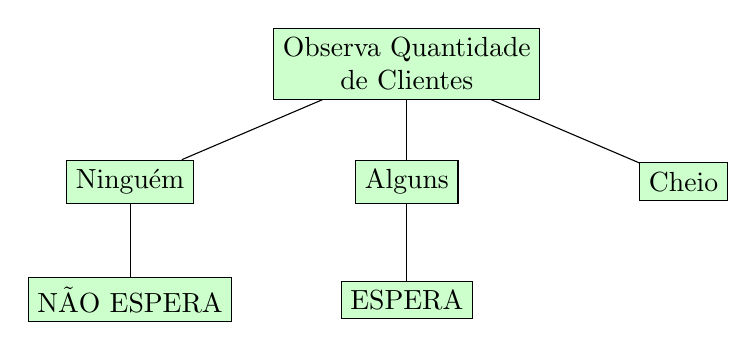
\begin{tikzpicture}[sibling distance=10em,
    every node/.style = {shape=rectangle, 
      draw, align=center,
      top color=green!20, bottom color=green!20}]]
    \node {Observa Quantidade \\ de Clientes}
        child { node {Ninguém} child { node {NÃO ESPERA}  } }
        child { node {Alguns} child { node {ESPERA} } }
        child { node {Cheio} };
  \end{tikzpicture}